\documentclass[12pt]{article}
\usepackage{amsmath}
\usepackage{graphicx}
\usepackage{hyperref}
\usepackage[utf8]{inputenc}
\usepackage{geometry}
\usepackage{mathtools}
\usepackage{empheq}
\usepackage{listings}
\usepackage{xcolor}
\usepackage{authblk}
\usepackage{subcaption}
\usepackage{svg}
\usepackage{minted}


\definecolor{LightGray}{gray}{0.9}

\graphicspath{ {./assets/} }
\geometry{margin=0.75in}

\title{CHEN 324 HW 6}
\author[1]{Zane Hernandez}
\author[2]{Bryce Gillilan}
\author[3]{Mark Levchenko}
\affil[1,2,3]{Group 11}
\date{24 March 2023}

\begin{document}
% \maketitle

\begin{enumerate}

%%%%%%%%%%%%%%%%%%%%%%%%%%%%%%%%%%%%%%%%%%%%%%%%%%%%%%%%%%%%%%%%%%%%%%%%
% Problem 1 %%%%%%%%%%%%%%%%%%%%%%%%%%%%%%%%%%%%%%%%%%%%%%%%%%%%%%%%%%%%
%%%%%%%%%%%%%%%%%%%%%%%%%%%%%%%%%%%%%%%%%%%%%%%%%%%%%%%%%%%%%%%%%%%%%%%%
\newpage
    \item Problem 26.3-1
    \[
        \alpha_{A/B} = \frac{\left(\frac{y_A}{x_A}\right)}{\left(\frac{y_B}{x_B}\right)} = \frac{\left(\frac{y_A}{x_A}\right)}{\left(\frac{1-y_A}{1-x_A}\right)}   
    \]

    Plot with data from Example 26.3-2:

    \begin{center}
        \includegraphics[width=0.8\textwidth]{assets/p1.png}
    \end{center}

%%%%%%%%%%%%%%%%%%%%%%%%%%%%%%%%%%%%%%%%%%%%%%%%%%%%%%%%%%%%%%%%%%%%%%%%
% Problem 2 %%%%%%%%%%%%%%%%%%%%%%%%%%%%%%%%%%%%%%%%%%%%%%%%%%%%%%%%%%%%
%%%%%%%%%%%%%%%%%%%%%%%%%%%%%%%%%%%%%%%%%%%%%%%%%%%%%%%%%%%%%%%%%%%%%%%%
\newpage
    \item Problem 26.3-2
    
    \begin{enumerate}
        \item 
        
        \begin{align*}
            \intertext{Fit equilibrium data from Example 26.3-2 to 4$^{\text{th}}$ order polynomial.}
            y(x) &= -3.806 x^4 + 10.185 x^3 - 10.141 x^2 + 4.749 x + 0.0101 \\
            \ln \left(\frac{L_1}{L_2}\right) &= \int_{x_2}^{x_1} \frac{dx}{y-x} \\
            & L_1 = 100 \\
            & x_1 = 0.6 \\
            \intertext{By mass balance}
            L_2 &= 60 \\
            0 &= \int_{x_2}^{0.6} \frac{dx}{-3.806 x^4 + 10.185 x^3 - 10.141 x^2 + 4.749 x + 0.0101 - x} - \ln \left(\frac{100}{60}\right) \\
            \intertext{Solve for $x_2$}
            \Aboxed{x_2 &= 0.407} \\
            \intertext{Material balance for A}
            L_1 x_1 &= L_2 x_2 + D y_{avg} \\
            100 \cdot 0.6 &= 60 \cdot 0.407 + 40 y_{avg} \\
            \Aboxed{y_{avg} &= 0.889}
        \end{align*}

        \item 
        \begin{align*}
            \intertext{Flash material balance}
            F x_F &= D y_D + W x_W \\
            y_D &= -3.806 x_W^4 + 10.185 x_W^3 - 10.141 x_W^2 + 4.749 x_W + 0.0101 \\
            100 \cdot 0.6 &= 40 \left(-3.806 x_W^4 + 10.185 x_W^3 - 10.141 x_W^2 + 4.749 x_W + 0.0101\right) + 60 x_W \\     
            \intertext{Solve for $x_W$}
            \Aboxed{x_W &= 0.429} \\
            y_D &= f(0.429) \\
            \Aboxed{y_D &= 0.856}
        \end{align*}

    \end{enumerate}

%%%%%%%%%%%%%%%%%%%%%%%%%%%%%%%%%%%%%%%%%%%%%%%%%%%%%%%%%%%%%%%%%%%%%%%%
% Problem 3 %%%%%%%%%%%%%%%%%%%%%%%%%%%%%%%%%%%%%%%%%%%%%%%%%%%%%%%%%%%%
%%%%%%%%%%%%%%%%%%%%%%%%%%%%%%%%%%%%%%%%%%%%%%%%%%%%%%%%%%%%%%%%%%%%%%%%
\newpage
    \item Problem 26.3-3 
    
    \begin{align*}
        \intertext{Fit equilibrium data from Tbale 26.1-1 to 4$^{\text{th}}$ order polynomial.}
        y(x) &= -0.417 x^4 + 1.493 x^3 - 2.361 x^2 + 2.285 x \\
        \ln \left(\frac{L_1}{L_2}\right) &= \int_{x_2}^{x_1} \frac{dx}{y-x} \\
        & L_1 = 100 \\
        & x_1 = 0.7 \\
        \intertext{By mass balance}
        L_2 &= 66.7 \\
        0 &= \int_{x_2}^{0.7} \frac{dx}{-0.417 x^4 + 1.493 x^3 - 2.361 x^2 + 2.285 x - x} - \ln \left(\frac{100}{66.7}\right) \\
        \intertext{Solve for $x_2$}
        \Aboxed{x_2 &= 0.632} \\
        \intertext{Material balance for A}
        L_1 x_1 &= L_2 x_2 + D y_{avg} \\
        100 \cdot 0.7 &= 66.7 \cdot 0.632 + 33.3 y_{avg} \\
        \Aboxed{y_{avg} &= 0.836}
    \end{align*}

%%%%%%%%%%%%%%%%%%%%%%%%%%%%%%%%%%%%%%%%%%%%%%%%%%%%%%%%%%%%%%%%%%%%%%%%
% Problem 4 %%%%%%%%%%%%%%%%%%%%%%%%%%%%%%%%%%%%%%%%%%%%%%%%%%%%%%%%%%%%
%%%%%%%%%%%%%%%%%%%%%%%%%%%%%%%%%%%%%%%%%%%%%%%%%%%%%%%%%%%%%%%%%%%%%%%%
\newpage
    \item Problem 26.4-3
    
    Use equilibrium data from Table 26.1-1
    
    \begin{enumerate}
        \item 
        \begin{align*}
            y(x) &= -0.417 x^4 + 1.493 x^3 - 2.361 x^2 + 2.285 x \\
            & x' = 0.5 \\
            y' = y(x') \\
            y' &= 0.713 \\
            R_m &= \frac{y_D - y'}{y' - x'} \\
            & y_D = 0.9 \\
            m &= \frac{0.9 - 0.713}{0.9 - 0.5} \\
            m &= 0.46 \\
            R_m &= \frac{m}{1 - m} \\
            R_m &= \frac{0.46}{1 - 0.46} \\
            \Aboxed{R_m &= 0.876}
        \end{align*}

        \item 
        
        Plot equilibrium line and 45$^\circ$ line. The operting lines are parallel to the 45$^\circ$ line at infinite reflux. 

        \begin{center}
            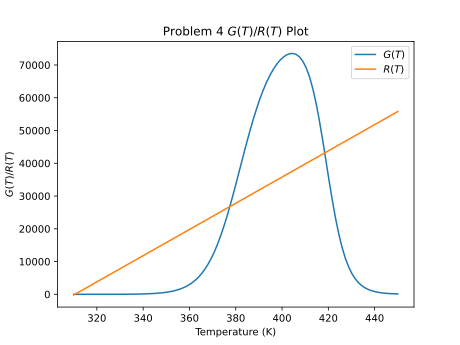
\includegraphics[width=0.8\textwidth]{assets/p4.png}
        \end{center}

        The total number of stages is 5. The minimum number of trays is 4 plus a reboiler.
    \end{enumerate}
    
\end{enumerate}
\end{document}
